%%%%%%%%%%%%%%%%%%%%%%%%%%%%%%%%%%%%%%%%%%%%%%%%%%%
%% P3: Phenomenology of Particle Physics                         
%%
%% Author:  André Rubbia                   		 
%%
%% Figure 2.15 Compilation by Geiger and Marsden of large-angle scattering of $\alpha$ particles by silver and gold foils.
%%
%% This work is licensed under the Creative Commons Attribution 4.0 International License. 
%% To view a copy of this license, visit http://creativecommons.org/licenses/by/4.0/ or 
%% send a letter to Creative Commons, PO Box 1866, Mountain View, CA 94042, USA.
%%
%% Data points taken from H.~Geiger and E.~Marsden, ``The laws of deflexion of $\alpha$ particles through
%%  large angles,'' Philosophical Magazine, vol. 25, no. 148, pp. 604-623 (1913).
%%
%%%%%%%%%%%%%%%%%%%%%%%%%%%%%%%%%%%%%%%%%%%%%%%%%%%

\documentclass[a4paper,10pt]{article}

\usepackage[T1]{fontenc}
\usepackage[utf8]{inputenc}
\usepackage{lmodern}
\usepackage[labelfont=bf]{caption}
\usepackage{upgreek}
\usepackage{amssymb}
\usepackage{amsmath}

\usepackage{tikz}
\usepackage{pgfplots}
\pgfplotsset{compat=1.17}
\usepgfplotslibrary{ternary}
\usepgfplotslibrary{fillbetween}
\usepgfplotslibrary{external}


\def\d{\mathrm{d}}

\begin{document}

%%%%%%%%%%%%%%%   FIGURE  %%%%%%%%%%%%%%%%%%%%%%%%%%%%%%
\begin{figure}[htb]
\begin{center}
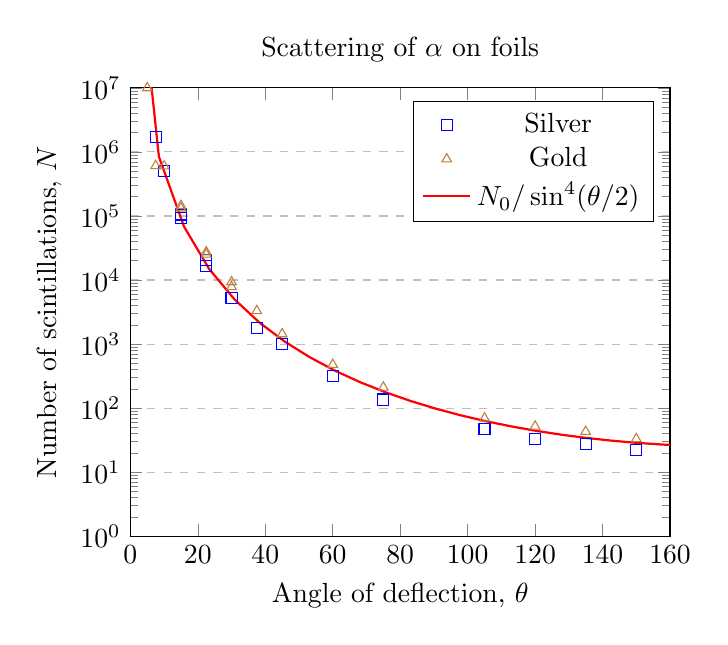
\begin{tikzpicture}[scale=1]
\begin{semilogyaxis}[
    title={Scattering of $\alpha$ on foils},
    xlabel={Angle of deflection, $\theta$},
    ylabel={Number of scintillations, $N$},
    xmin=0, xmax=160,
    ymin=1, ymax=1e7,
    xtick={0,20,40,60,80,100,120,140,160},
    ytick={1e0,1e1,1e2,1e3,1e4,1e5,1e6,1e7},
    legend pos=north east,
    ymajorgrids=true,
    grid style=dashed,
]
\addplot[
    color=blue,
    mark=square, only marks
    ]
    coordinates {
    (150,22.2)(135,27.4)(120,33)(105,47.3)(75,136)(60,320)(45,989)(37.5,1760)(30,5260)(22.5,20300)(15,105400)
    (30,5.3*1e3)(22.5,16.6*1e3)(15,93*1e3)(10,508*1e3)(7.5,1710*1e3)
    };
\addplot[
    color=brown,
    mark=triangle, only marks
    ]
    coordinates {
    (150,33.1)(135,43.0)(120,51.9)(105,69.5)(75,211)(60,477)(45,1435)(37.5,3300)(30,7800)(22.5,27300)(15,132000)
    (30,3.1*3e3)(22.5,8.4*3e3)(15,48.2*3e3)(10,200*3e3)(7.5,607*1e3)(5,3320*3e3)
    };
 \addplot[domain=1:180,
    color=red, thick]
    {0.25e2/sin(x/2)^4};
     \legend{Silver,Gold,$N_0/\sin^4(\theta/2)$}
\end{semilogyaxis}
\end{tikzpicture}
\caption{Compilation by Geiger and Marsden of large-angle scattering
of $\alpha$ particles by silver and gold foils.}
\end{center}
\end{figure}
%%%%%%%%%%%%%%%   END FIGURE  %%%%%%%%%%%%%%%%%%%%%%%%%%%%%%

\end{document}
